\subsubsection{2.5. Kết quả kiểm thử trên mô hình CNN + MGAT + mô hình phân lớp truyền thống với toàn bộ phương thức}
\indent\indent Để đánh giá khách quan chất lượng của các đặc trưng (features) được học bởi kiến trúc đồ thị, tôi thực hiện một thử nghiệm bổ sung thay thế bộ phân lớp học sâu (FastKAN/MLP) bằng các thuật toán máy học truyền thống.\vspace{0.3cm}

Cụ thể, tôi sử dụng mô hình đạt hiệu năng cao nhất ở kịch bản huấn luyện và kiểm thử trên toàn bộ phương thức, đó là DenseNet121 + MGAT + FastKAN. Mô hình này đóng vai trò như bộ trích xuất đặc trưng, với các vector đặc trưng tổng hợp từ tầng GAT cuối cùng (trước khi đi vào tầng FastKAN) được trích xuất và sử dụng làm dữ liệu đầu vào để huấn luyện các mô hình phân lớp cơ bản gồm KNN, Naive Bayes, Decision Tree, Random Forest, Logistic Regression và Linear SVC, trong đó phương pháp xử lý vector đặc trưng đã được đề cập ở mục 2.1.\vspace{0.3cm}

Bên dưới là bảng số liệu và biểu đồ thể hiện kết quả kiểm thử trung bình của các mô hình:
\begin{table}[H]
\centering
\caption{\centering Kết quả kiểm thử trung bình của các mô hình truyền thống (sử dụng đặc trưng từ DenseNet121 + MGAT + FastKAN)}
\label{tab:TraditionalModelsSummary}
\renewcommand{\arraystretch}{1.15}
\begin{tabular}{lcccc}
\hline
\textbf{Mô hình} & \textbf{Accuracy} & \textbf{Precision} & \textbf{Recall} & \textbf{F1-Score} \\
\hline
KNN (k = 1)                   & 0.8213 & 0.8289 & 0.8213 & 0.8022 \\
Gaussian NB                   & 0.7306 & 0.7210 & 0.7306 & 0.7142 \\
Decision Tree (max\_depth = 10) & 0.7556 & 0.7656 & 0.7556 & 0.7412 \\
Random Forest (n\_estimators = 20) & 0.8083 & 0.8108 & 0.8083 & 0.7859 \\
Logistic Regression (C = 10)      & 0.8370 & 0.8419 & 0.8370 & 0.8272 \\
Linear SVC (C = 0.01)             & 0.8676 & 0.8696 & 0.8676 & 0.8649 \\
\hline
{DenseNet121 + MGAT + FastKAN} & \textbf{0.9435} & \textbf{0.9477} & \textbf{0.9435} & \textbf{0.9438} \\
\hline
\end{tabular}
\end{table}

\begin{figure}[H]
    \centering
    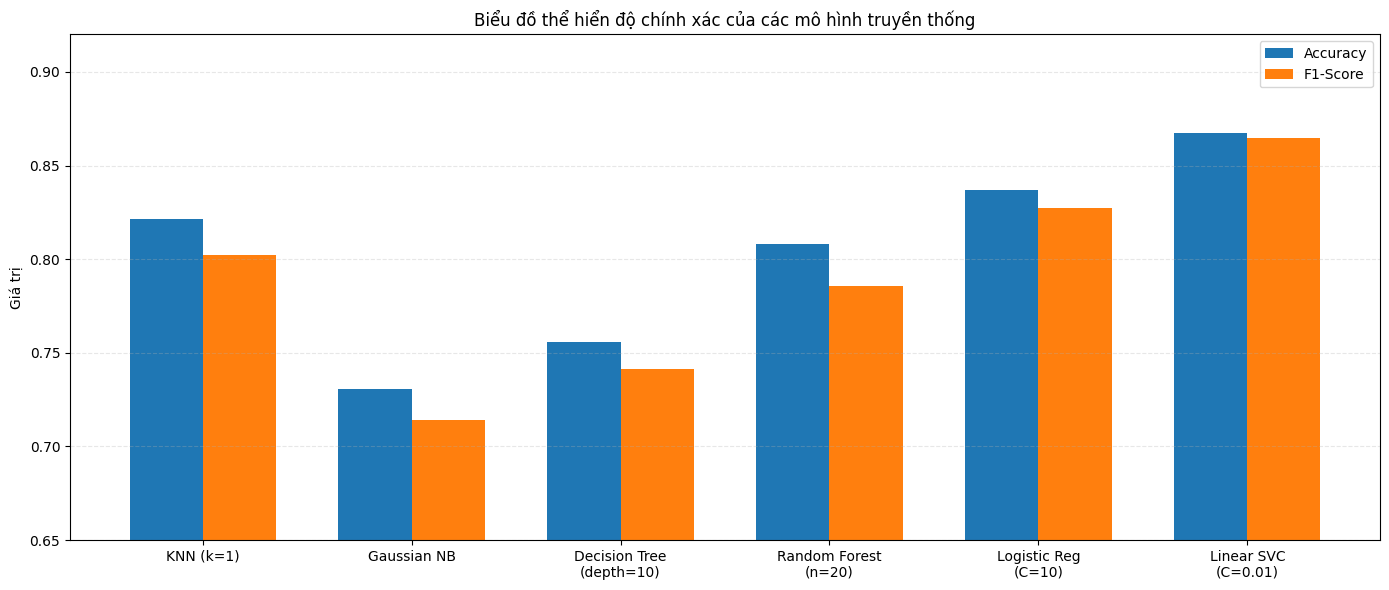
\includegraphics[width=\linewidth]{images/part-02/chap-03/sec-02/Tradition.png}
    \caption{\centering Biểu đồ thể hiện kết quả kiểm thử trung bình của các mô hình truyền thống (sử dụng đặc trưng từ DenseNet121 + MGAT + FastKAN)}
    \label{fig:KQTradition}
\end{figure}

\indent Dựa trên số liệu thu được từ bảng kết quả kiểm thử trung bình của các mô hình truyền thống, tôi rút ra các kết luận về chất lượng biểu diễn dữ liệu của mô hình đề xuất như sau:\vspace{-0.1cm}
\begin{itemize}[label={--}, itemsep=1pt]
    \item \textbf{Khả năng phân tách tuyến tính của không gian đặc trưng:} Kết quả của mô hình Linear SVC đạt độ chính xác 0.8676 cho thấy các vector đặc trưng đầu ra từ tầng MGAT có tính phân tách tuyến tính tương đối tốt. Điều này gợi ý rằng các mẫu dữ liệu cùng lớp đã được gom cụm trong không gian đặc trưng, tạo điều kiện thuận lợi cho các thuật toán phân lớp cơ bản hoạt động.
    \item \textbf{Vai trò trích xuất đặc trưng của MGAT:} Kết quả này xác nhận kiến trúc MGAT đã thực hiện được chức năng tổng hợp thông tin từ các phương thức dữ liệu rời rạc (hình ảnh, văn bản, âm thanh) thành các vector biểu diễn ngữ nghĩa thống nhất trước khi đi vào khâu phân lớp cuối cùng.
    \item \textbf{So sánh hiệu năng với FastKAN:} Vẫn tồn tại khoảng cách hiệu năng (khoảng 7-8\%) giữa Linear SVC so với FastKAN (đạt 0.9435). Điều này phản ánh giới hạn của các mô hình tuyến tính trong việc xử lý các biên quyết định phức tạp của dữ liệu di sản văn hóa. Các mẫu dữ liệu có độ nhập nhằng cao đòi hỏi khả năng biểu diễn phi tuyến linh hoạt hơn của FastKAN để đạt được độ chính xác cao hơn.
\end{itemize}